\subsection{simple-device-3.c}
\begin{frame}{\cod{simple-device-3.c}}{read/write}
\begin{itemize}
 \item read/write:
 \begin{itemize}
  \item \cod{copy\_to\_user}/\cod{copy\_from\_user}
  \item das Zusammenspiel:
  \begin{itemize}
   \item \cod{len} und \cod{*ofs}
  \end{itemize}
 \end{itemize}
\end{itemize}
\end{frame}

\begin{frame}[fragile]{read}
\begin{center}
 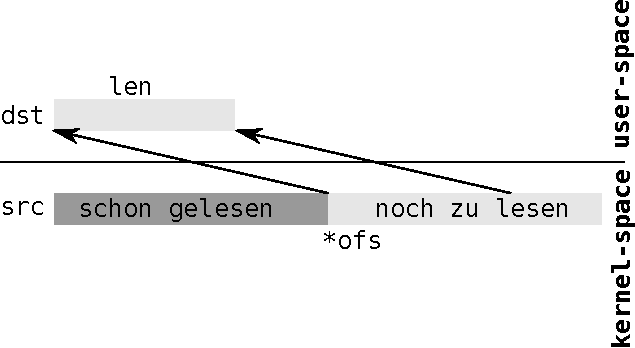
\includegraphics[width=0.875\textwidth]{user-kernel-space-read.pdf}
\end{center}
\vspace{-1.5cm}
\begin{lstlisting}
unsigned long copy_to_user(void __user *to, 
                           const void *from, 
                           unsigned long n)
\end{lstlisting}
\end{frame}

\begin{frame}[fragile]{write}
\begin{center}
 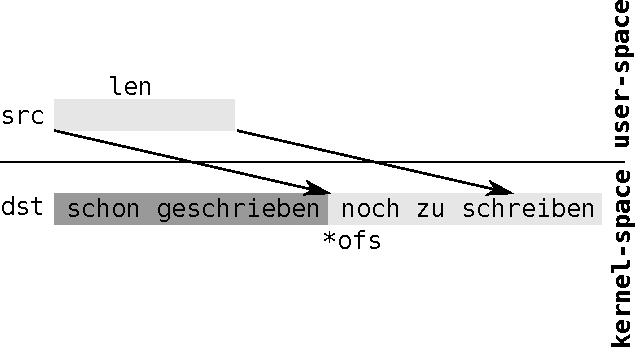
\includegraphics[width=0.875\textwidth]{user-kernel-space-write.pdf}
\end{center}
\vspace{-1.5cm}
\begin{lstlisting}
unsigned long copy_from_user(void *to, 
                                 const void __user *from, 
                                 unsigned long n)
\end{lstlisting}
\end{frame}
